
%% bare_conf.tex
%% V1.3
%% 2007/01/11
%% by Michael Shell
%% See:
%% http://www.michaelshell.org/
%% for current contact information.
%%
%% This is a skeleton file demonstrating the use of IEEEtran.cls
%% (requires IEEEtran.cls version 1.7 or later) with an IEEE conference paper.
%%
%% Support sites:
%% http://www.michaelshell.org/tex/ieeetran/
%% http://www.ctan.org/tex-archive/macros/latex/contrib/IEEEtran/
%% and
%% http://www.ieee.org/

%%*************************************************************************
%% Legal Notice:
%% This code is offered as-is without any warranty either expressed or
%% implied; without even the implied warranty of MERCHANTABILITY or
%% FITNESS FOR A PARTICULAR PURPOSE! 
%% User assumes all risk.
%% In no event shall IEEE or any contributor to this code be liable for
%% any damages or losses, including, but not limited to, incidental,
%% consequential, or any other damages, resulting from the use or misuse
%% of any information contained here.
%%
%% All comments are the opinions of their respective authors and are not
%% necessarily endorsed by the IEEE.
%%
%% This work is distributed under the LaTeX Project Public License (LPPL)
%% ( http://www.latex-project.org/ ) version 1.3, and may be freely used,
%% distributed and modified. A copy of the LPPL, version 1.3, is included
%% in the base LaTeX documentation of all distributions of LaTeX released
%% 2003/12/01 or later.
%% Retain all contribution notices and credits.
%% ** Modified files should be clearly indicated as such, including  **
%% ** renaming them and changing author support contact information. **
%%
%% File list of work: IEEEtran.cls, IEEEtran_HOWTO.pdf, bare_adv.tex,
%%                    bare_conf.tex, bare_jrnl.tex, bare_jrnl_compsoc.tex
%%*************************************************************************

% *** Authors should verify (and, if needed, correct) their LaTeX system  ***
% *** with the testflow diagnostic prior to trusting their LaTeX platform ***
% *** with production work. IEEE's font choices can trigger bugs that do  ***
% *** not appear when using other class files.                            ***
% The testflow support page is at:
% http://www.michaelshell.org/tex/testflow/



% Note that the a4paper option is mainly intended so that authors in
% countries using A4 can easily print to A4 and see how their papers will
% look in print - the typesetting of the document will not typically be
% affected with changes in paper size (but the bottom and side margins will).
% Use the testflow package mentioned above to verify correct handling of
% both paper sizes by the user's LaTeX system.
%
% Also note that the "draftcls" or "draftclsnofoot", not "draft", option
% should be used if it is desired that the figures are to be displayed in
% draft mode.
%
\documentclass[conference,a4paper]{IEEEtran}
% Add the compsoc option for Computer Society conferences.
%
% If IEEEtran.cls has not been installed into the LaTeX system files,
% manually specify the path to it like:
% \documentclass[conference]{../sty/IEEEtran}





% Some very useful LaTeX packages include:
% (uncomment the ones you want to load)


% *** MISC UTILITY PACKAGES ***
%
%\usepackage{ifpdf}
% Heiko Oberdiek's ifpdf.sty is very useful if you need conditional
% compilation based on whether the output is pdf or dvi.
% usage:
% \ifpdf
%   % pdf code
% \else
%   % dvi code
% \fi
% The latest version of ifpdf.sty can be obtained from:
% http://www.ctan.org/tex-archive/macros/latex/contrib/oberdiek/
% Also, note that IEEEtran.cls V1.7 and later provides a builtin
% \ifCLASSINFOpdf conditional that works the same way.
% When switching from latex to pdflatex and vice-versa, the compiler may
% have to be run twice to clear warning/error messages.






% *** CITATION PACKAGES ***
%
\usepackage{cite}
% cite.sty was written by Donald Arseneau
% V1.6 and later of IEEEtran pre-defines the format of the cite.sty package
% \cite{} output to follow that of IEEE. Loading the cite package will
% result in citation numbers being automatically sorted and properly
% "compressed/ranged". e.g., [1], [9], [2], [7], [5], [6] without using
% cite.sty will become [1], [2], [5]--[7], [9] using cite.sty. cite.sty's
% \cite will automatically add leading space, if needed. Use cite.sty's
% noadjust option (cite.sty V3.8 and later) if you want to turn this off.
% cite.sty is already installed on most LaTeX systems. Be sure and use
% version 4.0 (2003-05-27) and later if using hyperref.sty. cite.sty does
% not currently provide for hyperlinked citations.
% The latest version can be obtained at:
% http://www.ctan.org/tex-archive/macros/latex/contrib/cite/
% The documentation is contained in the cite.sty file itself.






% *** GRAPHICS RELATED PACKAGES ***
%
\ifCLASSINFOpdf
   \usepackage[pdftex]{graphicx}
  % declare the path(s) where your graphic files are
   \graphicspath{{figures/}}%{../jpeg/}}
  % and their extensions so you won't have to specify these with
  % every instance of \includegraphics
   \DeclareGraphicsExtensions{.pdf,.jpeg,.png}
\else
  % or other class option (dvipsone, dvipdf, if not using dvips). graphicx
  % will default to the driver specified in the system graphics.cfg if no
  % driver is specified.
  % \usepackage[dvips]{graphicx}
  % declare the path(s) where your graphic files are
  % \graphicspath{{../eps/}}
  % and their extensions so you won't have to specify these with
  % every instance of \includegraphics
  % \DeclareGraphicsExtensions{.eps}
\fi
% graphicx was written by David Carlisle and Sebastian Rahtz. It is
% required if you want graphics, photos, etc. graphicx.sty is already
% installed on most LaTeX systems. The latest version and documentation can
% be obtained at: 
% http://www.ctan.org/tex-archive/macros/latex/required/graphics/
% Another good source of documentation is "Using Imported Graphics in
% LaTeX2e" by Keith Reckdahl which can be found as epslatex.ps or
% epslatex.pdf at: http://www.ctan.org/tex-archive/info/
%
% latex, and pdflatex in dvi mode, support graphics in encapsulated
% postscript (.eps) format. pdflatex in pdf mode supports graphics
% in .pdf, .jpeg, .png and .mps (metapost) formats. Users should ensure
% that all non-photo figures use a vector format (.eps, .pdf, .mps) and
% not a bitmapped formats (.jpeg, .png). IEEE frowns on bitmapped formats
% which can result in "jaggedy"/blurry rendering of lines and letters as
% well as large increases in file sizes.
%
% You can find documentation about the pdfTeX application at:
% http://www.tug.org/applications/pdftex





% *** MATH PACKAGES ***
%
\usepackage[cmex10]{amsmath}
% A popular package from the American Mathematical Society that provides
% many useful and powerful commands for dealing with mathematics. If using
% it, be sure to load this package with the cmex10 option to ensure that
% only type 1 fonts will utilized at all point sizes. Without this option,
% it is possible that some math symbols, particularly those within
% footnotes, will be rendered in bitmap form which will result in a
% document that can not be IEEE Xplore compliant!
%
% Also, note that the amsmath package sets \interdisplaylinepenalty to 10000
% thus preventing page breaks from occurring within multiline equations. Use:
%\interdisplaylinepenalty=2500
% after loading amsmath to restore such page breaks as IEEEtran.cls normally
% does. amsmath.sty is already installed on most LaTeX systems. The latest
% version and documentation can be obtained at:
% http://www.ctan.org/tex-archive/macros/latex/required/amslatex/math/


\usepackage{siunitx}



% *** SPECIALIZED LIST PACKAGES ***
%
\usepackage{algorithmic}
% algorithmic.sty was written by Peter Williams and Rogerio Brito.
% This package provides an algorithmic environment fo describing algorithms.
% You can use the algorithmic environment in-text or within a figure
% environment to provide for a floating algorithm. Do NOT use the algorithm
% floating environment provided by algorithm.sty (by the same authors) or
% algorithm2e.sty (by Christophe Fiorio) as IEEE does not use dedicated
% algorithm float types and packages that provide these will not provide
% correct IEEE style captions. The latest version and documentation of
% algorithmic.sty can be obtained at:
% http://www.ctan.org/tex-archive/macros/latex/contrib/algorithms/
% There is also a support site at:
% http://algorithms.berlios.de/index.html
% Also of interest may be the (relatively newer and more customizable)
% algorithmicx.sty package by Szasz Janos:
% http://www.ctan.org/tex-archive/macros/latex/contrib/algorithmicx/




% *** ALIGNMENT PACKAGES ***
%
%\usepackage{array}
% Frank Mittelbach's and David Carlisle's array.sty patches and improves
% the standard LaTeX2e array and tabular environments to provide better
% appearance and additional user controls. As the default LaTeX2e table
% generation code is lacking to the point of almost being broken with
% respect to the quality of the end results, all users are strongly
% advised to use an enhanced (at the very least that provided by array.sty)
% set of table tools. array.sty is already installed on most systems. The
% latest version and documentation can be obtained at:
% http://www.ctan.org/tex-archive/macros/latex/required/tools/


%\usepackage{mdwmath}
%\usepackage{mdwtab}
% Also highly recommended is Mark Wooding's extremely powerful MDW tools,
% especially mdwmath.sty and mdwtab.sty which are used to format equations
% and tables, respectively. The MDWtools set is already installed on most
% LaTeX systems. The lastest version and documentation is available at:
% http://www.ctan.org/tex-archive/macros/latex/contrib/mdwtools/


% IEEEtran contains the IEEEeqnarray family of commands that can be used to
% generate multiline equations as well as matrices, tables, etc., of high
% quality.


%\usepackage{eqparbox}
% Also of notable interest is Scott Pakin's eqparbox package for creating
% (automatically sized) equal width boxes - aka "natural width parboxes".
% Available at:
% http://www.ctan.org/tex-archive/macros/latex/contrib/eqparbox/





% *** SUBFIGURE PACKAGES ***
%\usepackage[tight,footnotesize]{subfigure}
% subfigure.sty was written by Steven Douglas Cochran. This package makes it
% easy to put subfigures in your figures. e.g., "Figure 1a and 1b". For IEEE
% work, it is a good idea to load it with the tight package option to reduce
% the amount of white space around the subfigures. subfigure.sty is already
% installed on most LaTeX systems. The latest version and documentation can
% be obtained at:
% http://www.ctan.org/tex-archive/obsolete/macros/latex/contrib/subfigure/
% subfigure.sty has been superceeded by subfig.sty.


%\usepackage{graphicx}
%\graphicspath{{figures/}}
%\usepackage[caption=false]{caption}
%\usepackage[font=footnotesize]{subfig}
% subfig.sty, also written by Steven Douglas Cochran, is the modern
% replacement for subfigure.sty. However, subfig.sty requires and
% automatically loads Axel Sommerfeldt's caption.sty which will override
% IEEEtran.cls handling of captions and this will result in nonIEEE style
% figure/table captions. To prevent this problem, be sure and preload
% caption.sty with its "caption=false" package option. This is will preserve
% IEEEtran.cls handing of captions. Version 1.3 (2005/06/28) and later 
% (recommended due to many improvements over 1.2) of subfig.sty supports
% the caption=false option directly:
%\usepackage[caption=false,font=footnotesize]{subfig}
%
% The latest version and documentation can be obtained at:
% http://www.ctan.org/tex-archive/macros/latex/contrib/subfig/
% The latest version and documentation of caption.sty can be obtained at:
% http://www.ctan.org/tex-archive/macros/latex/contrib/caption/




% *** FLOAT PACKAGES ***
%
%\usepackage{fixltx2e}
% fixltx2e, the successor to the earlier fix2col.sty, was written by
% Frank Mittelbach and David Carlisle. This package corrects a few problems
% in the LaTeX2e kernel, the most notable of which is that in current
% LaTeX2e releases, the ordering of single and double column floats is not
% guaranteed to be preserved. Thus, an unpatched LaTeX2e can allow a
% single column figure to be placed prior to an earlier double column
% figure. The latest version and documentation can be found at:
% http://www.ctan.org/tex-archive/macros/latex/base/



%\usepackage{stfloats}
% stfloats.sty was written by Sigitas Tolusis. This package gives LaTeX2e
% the ability to do double column floats at the bottom of the page as well
% as the top. (e.g., "\begin{figure*}[!b]" is not normally possible in
% LaTeX2e). It also provides a command:
%\fnbelowfloat
% to enable the placement of footnotes below bottom floats (the standard
% LaTeX2e kernel puts them above bottom floats). This is an invasive package
% which rewrites many portions of the LaTeX2e float routines. It may not work
% with other packages that modify the LaTeX2e float routines. The latest
% version and documentation can be obtained at:
% http://www.ctan.org/tex-archive/macros/latex/contrib/sttools/
% Documentation is contained in the stfloats.sty comments as well as in the
% presfull.pdf file. Do not use the stfloats baselinefloat ability as IEEE
% does not allow \baselineskip to stretch. Authors submitting work to the
% IEEE should note that IEEE rarely uses double column equations and
% that authors should try to avoid such use. Do not be tempted to use the
% cuted.sty or midfloat.sty packages (also by Sigitas Tolusis) as IEEE does
% not format its papers in such ways.

% *** PDF, URL AND HYPERLINK PACKAGES ***
%
\usepackage[obeyspaces]{url}
\usepackage{hyperref}% http://ctan.org/pkg/hyperref
% url.sty was written by Donald Arseneau. It provides better support for
% handling and breaking URLs. url.sty is already installed on most LaTeX
% systems. The latest version can be obtained at:
% http://www.ctan.org/tex-archive/macros/latex/contrib/misc/
% Read the url.sty source comments for usage information. Basically,
% \url{my_url_here}.

% Advanced table environment
\usepackage{booktabs}



% *** Do not adjust lengths that control margins, column widths, etc. ***
% *** Do not use packages that alter fonts (such as pslatex).         ***
% There should be no need to do such things with IEEEtran.cls V1.6 and later.
% (Unless specifically asked to do so by the journal or conference you plan
% to submit to, of course. )


% correct bad hyphenation here
\hyphenation{op-tical net-works semi-conduc-tor ar-ti-ficial in-telli-gence conscious-thought}


\begin{document}
%
% paper title
% can use linebreaks \\ within to get better formatting as desired
%\title{Survey paper: \\Artificial Intelligence for optimisation of HVAC-systems}
\title{Autonomous F1/10-car using Artificial Intelligence }


% author names and affiliations
% use a multiple column layout for up to three different
% affiliations

%\author{\IEEEauthorblockN{Jens de Hoog}
%\IEEEauthorblockA{Department of Applied Engineering \\Electronics-ICT\\
%University of Antwerp\\
%Antwerp, Belgium\\
%jens.dehoog@student.uantwerpen.be}
%\and
%\IEEEauthorblockN{Maggy Goossens}
%\IEEEauthorblockA{Department of Applied Engineering \\Electronics-ICT\\
%University of Antwerp\\
%Antwerp, Belgium\\
%maggy.goossens@uantwerpen.be}
%\and
%\IEEEauthorblockN{Peter Hellinckx}
%\IEEEauthorblockA{Department of Applied Engineering \\Electronics-ICT\\
%University of Antwerp\\
%Antwerp, Belgium\\
%peter.hellinckx@uantwerpen.be}
%}

\author{
\IEEEauthorblockN{Jens de Hoog\IEEEauthorrefmark{1},
		Thomas Huybrechts\IEEEauthorrefmark{1}\IEEEauthorrefmark{4},
		Peter Hellinckx\IEEEauthorrefmark{1}\IEEEauthorrefmark{4}\\
	jens.dehoog@student.uantwerpen.be, thomas.huybrechts@uantwerpen.be, peter.hellinckx@uantwerpen.be}
	\\\IEEEauthorblockA{
	    \IEEEauthorrefmark{1}Department of Applied Engineering, Electronics-ICT, University of Antwerp, Belgium
	}
	\IEEEauthorblockA{
	    \IEEEauthorrefmark{4}IDLab, Department of Applied Engineering, University of Antwerp - iMinds, Belgium
	}
}

% make the title area
\maketitle

\begin{abstract}
%\boldmath
Insert abstract of the paper.

\end{abstract}
% IEEEtran.cls defaults to using nonbold math in the Abstract.
% This preserves the distinction between vectors and scalars. However,
% if the conference you are submitting to favors bold math in the abstract,
% then you can use LaTeX's standard command \boldmath at the very start
% of the abstract to achieve this. Many IEEE journals/conferences frown on
% math in the abstract anyway.

% no keywords

% For peer review papers, you can put extra information on the cover
% page as needed:
% \ifCLASSOPTIONpeerreview
% \begin{center} \bfseries EDICS Category: 3-BBND \end{center}
% \fi
%
% For peerreview papers, this IEEEtran command inserts a page break and
% creates the second title. It will be ignored for other modes.
\IEEEpeerreviewmaketitle



\section{Introduction}
Despite the fact that artificial intelligence (AI) is not a new concept, it has become increasingly popular these days. Its first goal was to let machines replicate the intelligence of a human being, but that goal appeared to be more difficult than researches thought it would be. Slow progress was made for the next years, but technology has become more powerful and the interest in AI increased again, especially in marketable aspects\cite{Brooks1991}. At present, AI is quite ubiquitous and is implemented in many topics, such as self-driving cars. \\

*Moet nog uitgebreid worden*

\section{Prerequisites}
%\subsection{F1/10-car}
%The F1/10-car consists of multiple sensors such as
The racecar was built using the online tutorials provided by the organisation, f1tenth.org. Although these tutorials are made for using the car on a race circuit, certain prerequisites have to be made. 

\subsection{Slow Accurate Driving}
%Hierin leg ik uit hoe het systeem om traag te rijden is gevorderd. Eerst gaat het over de ontwikkeling van de zogenaamde PWM-ception. Dit onderdeel krijgt natuurlijk een andere en deftigere naam. Ook komen hierin de problemen aan bod die ik heb ondervonden met het PWM-signaal. Dit omvat onder andere de Teensy die gaan lage frequenties met hoge dutycycles kan opwekken, of de ESC die geen hoge frequenties met lage dutycycles accepteert.

%Het systeem is ge\"{e}volueerd naar het systeem met de tellers en ticks. Ook dit systeem zal in beperkte mate uitgelegd worden.

First, the car cannot drive slowly with the current configuration, which is a challenge when debugging and testing software on the NVIDIA Jetson. Therefore, a solution has to be found. 

\subsubsection{Background}The Teensy microcontroller provides the signals for the steering servo and the Electronic Speed Control or ESC. These signals are independent square waves with a frequency of 100 Hz and a particular duty cycle, which ranges from 10\% to 20\% with 15\% as neutral value. When applying the neutral signals on both ESC and steering servo, the car does not move. The duty cycle of 10\% corresponds to steering to the left or driving backwards at full speed, whereas a value of 20\% corresponds to steering right or driving forward at maximum speed.

The numeric values used in the code for generating the PWM-signals are represented by a 16-bit integer. Thus, a duty cycle of 10\% accords to $\pm 6554$ and 20\% corresponds with $\pm 13108$. One can find that the matching value of 15\% is $\pm 9831$.

\subsubsection{Problem}A problem arises when the ESC-signal has a duty cycle which is a fraction higher than the neutral value. The motor does not drive instantly. Only at a particular numeric value of 10120 or at a duty cycle of 15.44189\%, the car starts driving at walking speed. Though, this speed is too fast when developing and debugging software. Hence, a certain deadzone exists between duty cycles 15\% and 15.44189\% which cannot be filled in by the hardware components. A software approach is needed in order to drive more slowly.

Figures \ref{fig:SlowDriving1}a and \ref{fig:SlowDriving1}b show the existing deadzone between the neutral state (shown by \ref{fig:SlowDriving1}a) and the state at which the car starts to drive (shown by \ref{fig:SlowDriving1}b). The figures are zoomed to make sure this difference is visible. As a result, the 

\begin{figure}
    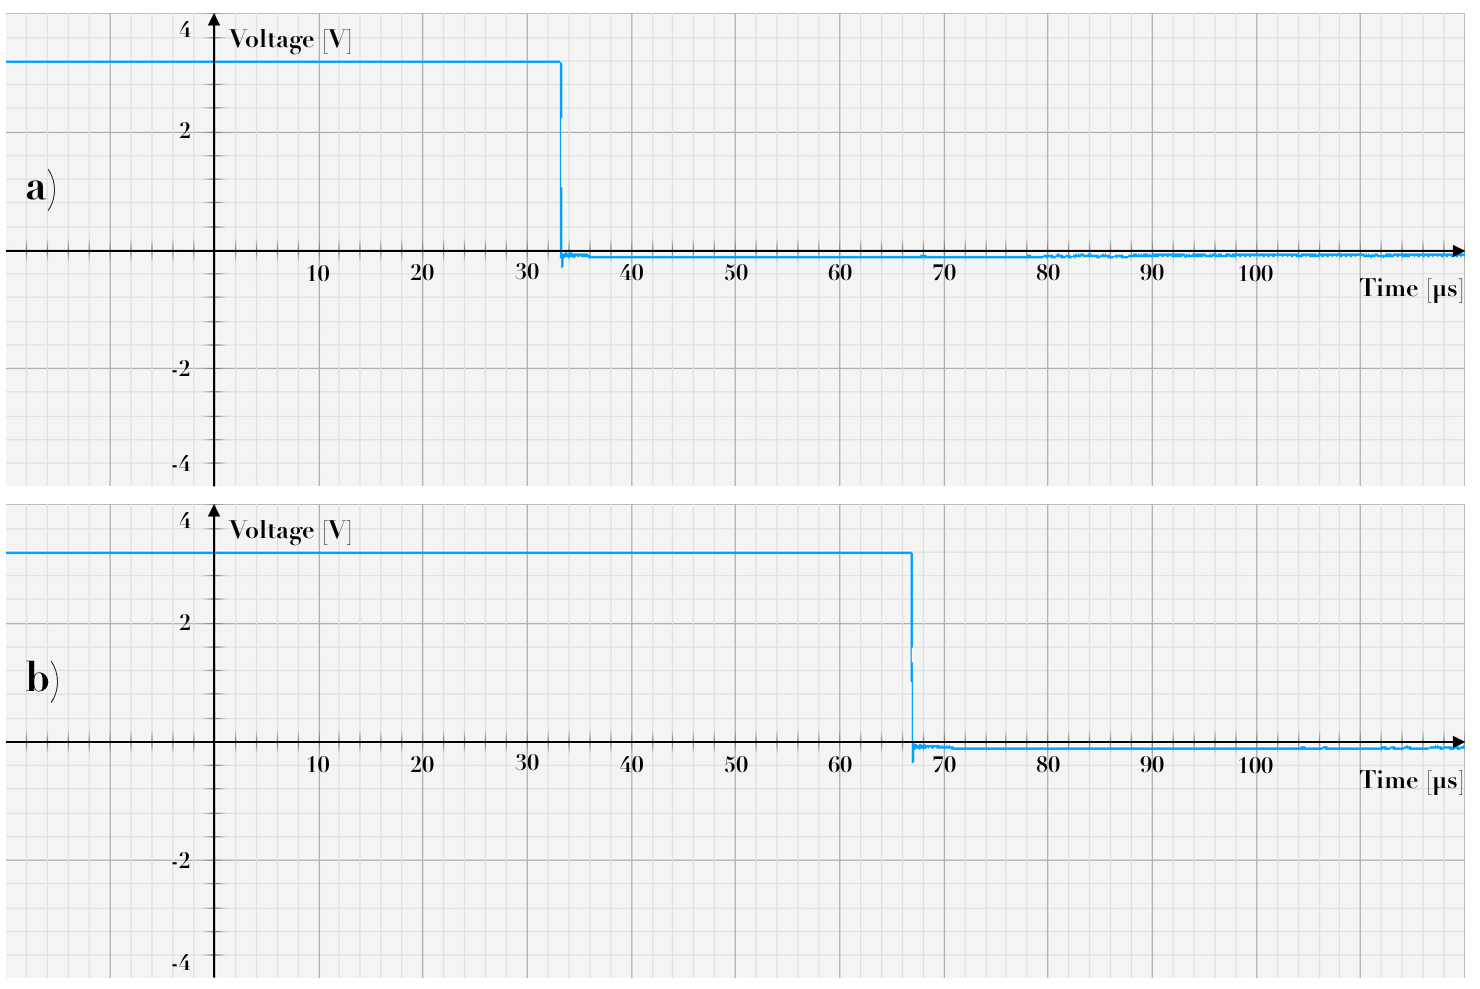
\includegraphics[width=\columnwidth]{SlowDriving1}
    \centering
    \caption{a) Shows the motorsignal in its neutral state. The duty cycle is 15\%. b) Shows the motorsignal at the moment when the car begins to drive. The corresponding duty cycle is 15.44189\%. Note that these figures are zoomed in order to display the difference between the two signals. Therefore, the complete period of the signal is not shown.}
    \label{fig:SlowDriving1}
\end{figure}

%Figure \ref{fig:SlowDriving1}a) shows the neutral state of the ESC. The duty cycle is equal to 15\%. Figure \ref{fig:SlowDriving1}b) displays the state at which the car begins to drive. This state corresponds to a duty cycle of 15.144189\%. The difference between these two signals is the deadzone

\subsubsection{Solutions} The general approach is to modulate the ESC-signal. More specifically, by switching the ESC on and off at a particular frequency, the speed can be regulated. The switching signal can be compared with a gate which allows the motorsignal to pass through. To generate such a signal, built-in timer mechanisms are needed. Luckily, the Teensy development board has three timers in its processor which can be accessed with low-level registers. Paul Stoffregen built a library which carries out the timer functions. This library is a fork of the original library for Arduino and implements multiple optimisations, along with support for more hardware configurations. \\

\noindent The first concept dealt with a PWM-signal which would modulate the ESC-controlsignal. The motor controller was turned on and off using the generated square wave. By varying the duty cycle of that wave, the active time of the ESC varied with it.

%\noindent \#\#\# ACTUAL IMPLEMENTATION TOEVOEGEN \#\#\#
A square wave signal was generated by using the aforementioned timers. When a square wave with a fixed duty cycle of 50\% is generated, an Interrupt Service Routine (ISR) can be connected which will be executed every time the pulse is high. When a signal with a variable duty cycle is produced, no ISR can be attached. The solution for this problem was to bound the signal to a GPIO-pin on which an ISR is connected. Thus, every time the pin goes high due to the PWM-signal, the ISR is executed. Inside this ISR, the ESC is alternately turned on and off.

Although this solution should work in theory, it appeared to be more difficult in practice because of limitations of the hardware components. First, the speed controller does not accept the signal at a high switching frequency with a low duty cycle. Besides that, the Teensy board cannot generate signals at a low switching rate with a high duty cycle. \\

%\noindent \#\#\# EXPLANATIONS TOEVOEGEN \#\#\#

\noindent The second concept takes a different approach. Instead of generating a switching signal with a fixed frequency and a variable duty cycle, a signal is generated with a fixed duty cycle of 50\% and a variable frequency. When the car needs to speed up, the frequency of that signal is decreased. Thus, the ESC has more time to increase the motor speed and the car will drive faster. By increasing the switching rate, the motor has less time to accelerate by which the car will slow down.

This approach is implemented by using the same timers of the previous approach. Instead of directly changing the timer frequency, the timer frequency is fixed at 100 Hz and generates interrupts at that rate. The ISR increments a counter which resets when a certain limit is reached. This limit value is set when the ESC-signal is located inside the deadzone. Depending on the specific location within that deadzone, the value of the limit is calculated. When the counter inside the ISR resets, the ESC is either turned on or off by sending the appropriate controller signal. In other words, by increasing or decreasing the limit value of the counter, the period by which the ESC is turned on or off is varying in the same way.
%a toggle is switched from '\textit{True}' to '\textit{False}' or vice versa. If that toggle is equal to '\textit{True}', the controller signal with a duty cycle of 15.44189\% is sent by which the car begins to drive. When the toggle is equal to '\textit{False}', the neutral signal is sent, thus the ESC does not power the motor anymore. In other words, 
%When the ESC-signal is located inside the deadzone, a particular parameter is set. This parameter corresponds to the threshold which resets the counter in the interrupt handler. When the ESC-signal is located inside the deadzone, a particular threshold is set. A counter is incremented in the Interrupt Service HandlerISR is reset when the 

\subsection{Driving at constant speed}
Het is een handigheid om op een hoger abstractieniveau "Ik wil 5km/u rijden" te kunnen zeggen. Dit komt vooral van pas bij de artificiële intelligentie. Daarom moet er een systeem gebouwd worden dat het rijden tegen constante snelheid voorziet. Dat systeem wordt in dit deel uitgelegd. De lezer ontdekt welke technieken ik heb geprobeerd en welke uiteindelijk gekozen is.

\subsection{Calculations}
Hierin vertel ik welke berekeningen gemaakt moeten worden om proper te kunnen rijden. Mooie voorbeelden zijn het throttlen en sturen voor het rijden op de ideale racelijn.

\section{Artificial Intelligence}
\subsection{Introduction and definitions}
%\subsubsection{Definitions}
The subject 'Artificial Intelligence' has many definitions, but Davis preferred this one: "There are a number of cognitive tasks that people do easily---often, indeed, with no consciousthought at all---but that it is extremely hard to program on computers. Artificial intelligence, as I define it, is the study of getting computers to carry out these tasks."\cite{Davis2014} Copeland stated another definition: "Artificial Intelligence is usually defined as the science of making computers do things that require intelligence when done by humans." \cite{Cop2000}\\

According to the research of Tk{\'{a}}{\v{c}} et al.\cite{Tkac2015}, artificial neural networks are structures which were built to match the aggregation of knowledge in a human nerve system. These artificial structures can solve non-linear problems which are extremely hard to solve by a conventional computational structure. Because of the flexibility, sturdiness and efficiency, these artificial neural networks are gaining popularity in different sorts of applications such as pattern recognition systems and financial utilisations.\cite{yegnanarayana2009artificial,Tkac2015}\\

*Kan nog uitgebreid worden*

\subsection{Applied on F1/10-car}
In dit deel praat ik over hoe AI in mijn systeem is ge\"{i}ntegreerd en hoe het concept in z'n werking gaat. Hoe de sensoren, ROS en de AI samenwerken, wordt hier uitgelegd met behulp van blokschema's en flowcharts. 

\subsection{Implementation}
Dit onderdeel handelt over de exacte implementatie, zonder stukken code te laten zien. Hier vertel ik over hoe het gekozen framework (bijvoorbeeld TensorFlow) in elkaar gestoken is. Het verschil met de vorige paragraaf is dat daar de AI gezien wordt als een zwarte doos die verbonden wordt met andere onderdelen. In dit deel wordt die zwarte doos opengetrokken en ga ik kijken naar de binnenkant van de AI. Zoals ik reeds zei komen hierin geen stukken code, maar eerder de concepten binnen de AI.

Ook kunnen hier designkeuzes naar voren komen, zoals welk framework ik heb gekozen en waarom. 

\section{Results}
In dit deel komen de resultaten naar boven van mijn masterproef. Hierin vertel ik hoe het autonoom rijden zijn werk doet en wat ik ermee behaald heb. Zo kan ik vertellen over de parcoursen die de auto heeft afgelegd en hoe de wagen dit tot een einde heeft gebracht. 

\section{Further Research}
Dit deel handelt over het onderzoek dat nog verricht moet worden om een volledig autonome auto te verkrijgen. Dit kan gaan van objectdetectie met de LiDAR-sensor tot interactie met andere wagens met oog op racen.

\section{Conclusion}
De conclusie van dit thesis wordt hierin verwerkt. Wat er exact in zal komen, weet ik nog niet precies. Ten eerste kan er iets gezegd worden over de voorbereidingen die getroffen moesten worden vooraleer de AI zijn werk kon doen. Als tweede kan er verteld worden over de AI zelf en hoe deze opgelost is, en of dit een goeie oplossing bleek te zijn. Als laatste kan er iets in komen over het verdere onderzoek dat nog moet gebeuren. 
% trigger a \newpage just before the given reference
% number - used to balance the columns on the last page
% adjust value as needed - may need to be readjusted if
% the document is modified later
%\IEEEtriggeratref{8}
% The "triggered" command can be changed if desired:
%\IEEEtriggercmd{\enlargethispage{-5in}}

% references section

% can use a bibliography generated by BibTeX as a .bbl file
% BibTeX documentation can be easily obtained at:
% http://www.ctan.org/tex-archive/biblio/bibtex/contrib/doc/
% The IEEEtran BibTeX style support page is at:
% http://www.michaelshell.org/tex/ieeetran/bibtex/
%\bibliographystyle{IEEEtran}
% argument is your BibTeX string definitions and bibliography database(s)
%\bibliography{IEEEabrv,../bib/paper}
%
% <OR> manually copy in the resultant .bbl file
% set second argument of \begin to the number of references
% (used to reserve space for the reference number labels box)

%\begin{thebibliography}{1}

%\bibitem{IEEEhowto:kopka}
%H.~Kopka and P.~W. Daly, \emph{A Guide to \LaTeX}, 3rd~ed.\hskip 1em plus
%  0.5em minus 0.4em\relax Harlow, England: Addison-Wesley, 1999.

%\end{thebibliography}
\newpage
\bibliographystyle{plain}
\bibliography{bibliography.bib}
%\bibliography{bibliography.bib}




% that's all folks
\end{document}